% !TeX root = report.tex
\documentclass{article}

\usepackage{listings}
\lstset{
    basicstyle=\ttfamily\footnotesize,
    showspaces=false,
    showstringspaces=false,
    numbers=left,
    frame=single
}

\usepackage{xcolor}
\usepackage{subcaption}
\usepackage{hyperref}
\usepackage{mathtools}

\usepackage{tikz}
\usetikzlibrary{3d}

\title{Modeling and Analysis of Robotic Arm of 6 DOF}
\author{***REMOVED*** \\ ***REMOVED***}

\begin{document}

\maketitle
\tableofcontents

\section{Description of the Problem}

% 随着工业自动化的大规模发展,机械臂在生产中得到了大规模的使用。
With the large-scale development of industrial automation, robotic arms have seen a large scale usage in production.
% 在众多机械臂中,三自由度机械臂凭借结构简单、控制容易以及造价低廉等优势受到青睐,因此也成为重要的研究对象。
Among various types of robotic arms, three-degree-of-freedom (DOF) robotic arms are favored due to their simple structure, easy control, and low cost, and therefore have become an important research object.

% 本技术报告将对一个经典的三自由度机械臂以及机械臂末端安装的三自由度机械手进行运动学分析、动力学分析和控制仿真。
This technical report will conduct forward and inverse kinematic analysis, dynamics analysis and control simulation of a classic three-degree-of-freedom robotic arm with a three-degree-of-freedom manipulator installed at the end of the arm.
% 该机械臂总共具有六个自由度,能够在三维空间中自由运动,实现指定的目标。
This robotic arm system has therefore a total of six degrees of freedom and can move freely in three-dimensional space to achieve specified goals.

\subsection{Model of the Arm}

% !TeX root = ..\report.tex

\begin{figure}[ht]
    \centering
    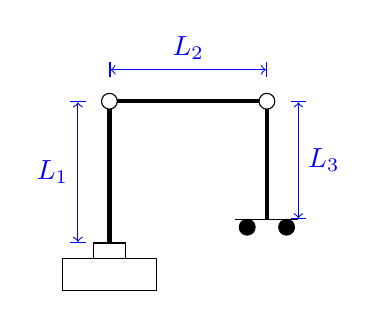
\begin{tikzpicture}
        % Arm 1 and foundation
        \draw (0.6, 0) rectangle (-0.6, -0.4);
        \draw (0.2, 0.2) rectangle (-0.2, 0);
        \draw [ultra thick] (0, 0.2) -- (0, 2);

        % Arm 2 and joint
        \draw [ultra thick] (0, 2) -- (2, 2);
        \draw [fill=white] (0, 2) circle [radius=0.1];
        
        % Arm 3 and joint
        \draw [ultra thick] (2,2) -- (2,0.5);
        \draw [fill=white] (2,2) circle [radius=0.1];
        \draw (1.6, 0.5) -- (2.4, 0.5);
        \draw [fill=black] (1.75, 0.4) circle [radius=0.1];
        \draw [fill=black] (2.25, 0.4) circle [radius=0.1];

        % Annotations
        \draw [|<->|, blue] (-0.4, 0.2) -- (-0.4, 2) node [pos=0.5, left] {$L_1$};
        \draw [|<->|, blue] (0, 2.4) -- (2, 2.4) node [pos=0.5, above] {$L_2$};
        \draw [|<->|, blue] (2.4, 2) -- (2.4, 0.5) node [pos=0.5, right] {$L_3$};
    \end{tikzpicture}
    \caption{机械臂主体部分示意图}
    \label{fig:robotic-arm-schema}
\end{figure}


% 本报告研究的机械臂系统由两个部分组成,第一个部分为具有三个旋转关节的三自由度机械臂,能够实现较大范围的自由运动;
The robotic arm system studied in this report consists of two parts.
The first part is a three-degree-of-freedom robotic arm with three rotating joints,
which can achieve a wide range of free movement;
% 第二个部分为机械臂末端安装的机械手型装置,该手型装置也具有三个自由度,能够实现对手持仪器的精密操作。
The second part is a manipulator-type device installed at the end of the robotic arm.
This hand-type device also has three degrees of freedom and can achieve precise operation of handheld instruments.
% 该机械手型装置可视为一个三自由度关节,也视为三个紧邻的单自由度关节。
The manipulator-type device can be viewed as a three-degree-of-freedom joint or as three adjacent single-degree-of-freedom joints.
% 由于机械手的质量相对于机械臂主体可忽略,在动力学分析中可以不对后三个关节进行建模。
Since the mass of the manipulator is negligible relative to the main body of the manipulator, the last three joints are not modeled in the dynamics analysis.
% 机械臂主体部分的示意图见图\ref{fig:robotic-arm-schema}。
The schematic diagram of the main part of the robotic arm is shown in the \autoref{fig:robotic-arm-schema}.

\section{Kinematic Model}

% 我们使用机器人学中广泛应用的\emph{Denavit-Hartenberg 方法}为每一个关节分配固连坐标系并进行运动学分析。
We use the \emph{Denavit-Hartenberg method}, which is widely used in robotics, to assign a affixed coordinate system to each joint and perform kinematic analysis.
% 按照以下约定选择和每个关节$i$与连杆$\{i\}$固连的坐标系:
The fixed frame of joint $i$ and link $\{i\}$ is constructed with the following convention:
\begin{enumerate}
    % \item 坐标系的Z轴$\hat Z_i$与$i$号关节方向重合;
    \item The Z axis of the frame $\hat Z_i$ is identical to the axis of joint $i$;
    % \item 原点选择在连杆两端关节轴线的公垂线与$i$号关节的轴线交点处;
    \item The origin is selected to be the intersection of the common perpendicular of the joint axes at both ending joints of the link and the axis of joint $i$;
    % \item X轴$\hat X_i$沿公垂线指向$i+1$号关节,若公垂线长度为零,则选择$\hat Z_i$与$\hat Z_{i+1}$构成的平面的法线;
    \item The X axis $\hat X_i$ points to joint $i+1$ along the common perpendicular, and be its length zero, the normal of the plane constructed by $\hat Z_i$ and $\hat Z_{i+1}$;
    % \item 按组成右手坐标系的原则选择Y轴$\hat Y_i$。
    \item The Y axis $\hat Y_i$ is selected so that the frame is right-handed.
\end{enumerate}
% 分配的坐标系如图\ref{fig:affixed-frame}所示。
Affixed frames on the arm are shown in \autoref{fig:affixed-frame}.

% !TeX root = ..\report.tex

\begin{figure}[ht]
    \centering
    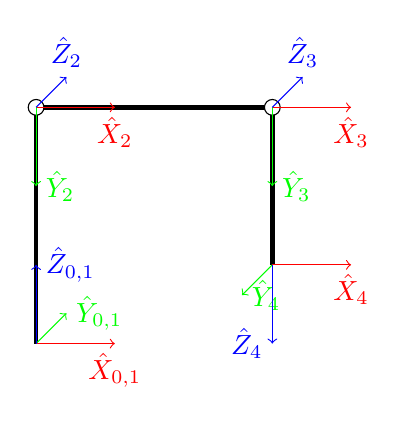
\begin{tikzpicture}
        % Arm 1
        \draw [ultra thick] (0, 0) -- (0, 3);

        \draw [->, red] (0,0,0) -- (1,0,0) node [below] {$\hat X_{0,1}$};
        \draw [->, green] (0,0,0) -- (0,0,-1) node [right] {$\hat Y_{0,1}$};
        \draw [->, blue] (0,0,0) -- (0,1,0) node [right] {$\hat Z_{0,1}$};

        % Arm 2
        \draw [ultra thick] (0, 3) -- (3, 3);
        \draw [fill=white] (0, 3) circle [radius=0.1];
        \draw [->, red] (0,3,0) -- (1,3,0) node [below] {$\hat X_2$};
        \draw [->, green] (0,3,0) -- (0,2,0) node [right] {$\hat Y_2$};
        \draw [->, blue] (0,3,0) -- (0,3,-1) node [above] {$\hat Z_2$};

        % Arm 3 and joint
        \draw [ultra thick] (3,3) -- (3,1);
        \draw [fill=white] (3,3) circle [radius=0.1];
        \draw [->, red] (3,3,0) -- (4,3,0) node [below] {$\hat X_3$};
        \draw [->, green] (3,3,0) -- (3,2,0) node [right] {$\hat Y_3$};
        \draw [->, blue] (3,3,0) -- (3,3,-1) node [above] {$\hat Z_3$};
        
        % Frame 4
        \draw [->, red] (3,1,0) -- (4,1,0) node [below] {$\hat X_4$};
        \draw [->, green] (3,1,0) -- (3,1,1) node[right] {$\hat Y_4$};
        \draw [->, blue] (3,1,0) -- (3,0,0) node[left] {$\hat Z_4$};
    \end{tikzpicture}
    \caption{固连坐标系分配}
    \label{fig:affixed-frame}
\end{figure}


% 按照指定的方法分配每个关节的固连坐标系后,可得出每个关节的 Denavit-Hartenberg 参数。
After determining affixed frames of each joint, Denavit-Hartenberg parameters of each joint can be acquired:
\begin{enumerate}
    % \item $\alpha_i$是轴$\hat Z_i$与$\hat Z_{i+1}$绕$\hat X_i$方向的夹角;
    % \item $a_i$是轴$\hat Z_i$与$\hat Z_{i+1}$沿$\hat X_i$方向的距离;
    % \item $d_i$是轴$\hat X_{i-1}$与$\hat X_i$沿$\hat Z_i$方向的距离;
    % \item $\theta_i$是轴$\hat X_{i-1}$与$\hat X_i$绕$\hat Z_i$方向的夹角。
    \item $\alpha_i$ is the angle between axis $\hat Z_i$ and $\hat Z_{i+1}$ around the direction of $\hat X_i$;
    \item $a_i$ is the distance between axis $\hat Z_i$ and $\hat Z_{i+1}$ along the $\hat X_i$ direction;
    \item $d_i$ is the distance between axis $\hat X_{i-1}$ and $\hat X_i$ along the $\hat Z_i$ direction;
    \item $\theta_i$ is the angle between axis $\hat X_{i-1}$ and $\hat X_i$ around the direction of $\hat Z_i$.
\end{enumerate}
% 计算的参数如表\ref{tab:DH-params}所示。
Such parameters are shown in \autoref{tab:DH-params}.

\begin{table}[ht]
    % \caption{Denavit-Hartenberg参数}
    \caption{Denavit-Hartenberg Parameters}
    \label{tab:DH-params}
    \centering
    \begin{tabular}{c|cccc}
        \hline
        & $\alpha_{i-1}$ & $a_{i-1}$ & $d_i$ & $\theta_i$ \\
        \hline
        1 & $0$ & $0$ & $0$ & $\theta_1$ \\
        2 & $-\frac{\pi}{2}$ & $L_1$ & $0$ & $\theta_2$ \\
        3 & $0$ & $L_2$ & $0$ & $\theta_3$ \\
        4 & $-\frac{\pi}{2}$ & $L_3$ & $0$ & $\theta_4$\\
        5 & $\frac{\pi}{2}$ & $0$ & $0$ & $\theta_5$\\
        6 & $-\frac{\pi}{2}$ & $0$ & $0$ & $\theta_6$\\ \hline
    \end{tabular}
\end{table}

\subsection{Forward Kinematics}

% 利用 Denavit-Hartenberg 参数,相邻两个坐标系之间的变换矩阵可以非常容易地表示出来,按照约定,有
With the help of Denavit-Hartenberg parameters, the transform matrix between adjacent frames can be evaluated easily.
Following the convention, we have
\[
    \begin{aligned}
        \prescript{i-1}{i}{T}
        &= R_X (\alpha_{i-1}) D_X (a_{i-1}) R_Z (\theta_i) D_Z (d_i) \\
        &= \begin{bmatrix}
            \cos \theta_i & - \sin \theta_i & 0 & \alpha_{i-1} \\
            \sin \theta_i \cos \alpha_{i-1} & \cos \theta_i \cos \alpha_{i-1} & - \sin \alpha_{i-1} & - \sin \alpha_{i-1} d_i \\
            \sin \theta_i \sin \alpha_{i-1} & \cos \theta_i \sin \alpha_{i-1} & \cos \alpha_{i-1} & \cos \alpha_{i-1} d_i \\
            0 & 0 & 0 & 1
        \end{bmatrix}
    \end{aligned}
\]

% 从而我们可以计算所有相邻坐标系的变换矩阵
Therefore all transform matrix of adjacent frames are determined as follows.
\[
    \prescript{0}{1}{T} =
    \begin{bmatrix}
        \cos \theta_1 & - \sin \theta_1 & 0 & 0 \\
        \sin \theta_1 & \cos \theta_1 & 0 & 0 \\
        0 & 0 & 1 & 0 \\
        0 & 0 & 0 & 1
    \end{bmatrix}
\]

\[
    \prescript{1}{2}{T} =
    \begin{bmatrix}
        \cos \theta_2 & - \sin \theta_2 & 0 & L_1 \\
        0 & 0 & 1 & 0 \\
        -\sin \theta_2 & - \cos \theta_2 & 0 & 0 \\
        0 & 0 & 0 & 1
    \end{bmatrix}
\]

\[
    \prescript{2}{3}{T} =
    \begin{bmatrix}
        \cos \theta_3 & - \sin \theta_3 & 0 & L_2 \\
        \sin \theta_3 & \cos \theta_3 & 0 & 0 \\
        0 & 0 & 1 & 0 \\
        0 & 0 & 0 & 1
    \end{bmatrix}
\]

\[
    \prescript{3}{4}{T} =
    \begin{bmatrix}
        \cos \theta_4 & - \sin \theta_4 & 0 & L_3 \\
        0 & 0 & 1 & 0 \\
        -\sin \theta_4 & - \cos \theta_4 & 0 & 0 \\
        0 & 0 & 0 & 1
    \end{bmatrix}
\]

\[
    \prescript{4}{5}{T} =
    \begin{bmatrix}
        \cos \theta_5 & - \sin \theta_5 & 0 & 0 \\
        0 & 0 & -1 & 0 \\
        \sin \theta_5 & \cos \theta_5 & 0 & 0 \\
        0 & 0 & 0 & 1
    \end{bmatrix}
\]

\[
    \prescript{5}{6}{T} =
    \begin{bmatrix}
        \cos \theta_6 & - \sin \theta_6 & 0 & 0 \\
        0 & 0 & 1 & 0 \\
        -\sin \theta_6 & - \cos \theta_6 & 0 & 0 \\
        0 & 0 & 0 & 1
    \end{bmatrix}
\]

% 然后我们可以利用矩阵乘法计算任何两个关节坐标系之间的变换。
Then transform between two arbitrary frames can be determined by matrix multiplication.
% 首先考虑机械手外部的变换,即从坐标系$1$到坐标系$3$的变换:
We consider firstly the transform without the hand manipulater, that is the transfrom from frame 1 to frame 3:
\[
    \prescript{1}{3}{T} = \prescript{1}{2}{T} \prescript{2}{3}{T} =
    \begin{bmatrix}
        \cos{\left( {{\theta }_3}+{{\theta }_2}\right) } & -\sin{\left( {{\theta }_3}+{{\theta }_2}\right) } & 0 & {L_2} \cos{ {{\theta }_2} }+{L_1}\\
        0 & 0 & 1 & 0\\
        -\sin{\left( {{\theta }_3}+{{\theta }_2}\right) } & -\cos{\left( {{\theta }_3}+{{\theta }_2}\right) } & 0 & - {L_2} \sin{ {{\theta }_2} } \\
        0 & 0 & 0 & 1
    \end{bmatrix}
\]
Therefore,
\[
    \prescript{0}{3}{T} =
    \begin{bmatrix}
        \cos \theta_1 \cos{\left( {{\theta }_3}+{{\theta }_2}\right) } & - \cos \theta_1 \sin{\left( {{\theta }_3}+{{\theta }_2}\right) }  & -\sin \theta_1 & \cos \theta_1 \left( {L_2} \cos\theta_2+{L_1}\right) \\
            \sin \theta_1 \cos{\left( {{\theta }_3}+{{\theta }_2}\right) } & - \sin \theta_1 \sin{\left( {{\theta }_3}+{{\theta }_2}\right) }  & \cos \theta_1 & \sin \theta_1 \left( {L_2} \cos\theta_2+{L_1}\right) \\
            -\sin{\left( {{\theta }_3}+{{\theta }_2}\right) } & -\cos{\left( {{\theta }_3}+{{\theta }_2}\right) } & 0 & - {L_2} \sin \theta_2 \\
            0 & 0 & 0 & 1
    \end{bmatrix}
\]

% 然后考虑机械手内部的变换,即从坐标系$4$到坐标系$6$的变换:
Then we consider the transform within the hand manipulater, that is from frame 4 to frame 6:
\[
    \prescript{4}{6}{T} = \prescript{4}{5}{T} \prescript{5}{6}{T} =
    \begin{bmatrix}\cos{ {{\theta }_5} } \cos{ {{\theta }_6} } & - \cos{ {{\theta }_5} } \sin{ {{\theta }_6} }  & -\sin{ {{\theta }_5} } & 0\\
        \sin{ {{\theta }_6} } & \cos{ {{\theta }_6} } & 0 & 0\\
        \sin{ {{\theta }_5} } \cos{ {{\theta }_6} } & - \sin{ {{\theta }_5} } \sin{ {{\theta }_6} }  & \cos{ {{\theta }_5} } & 0\\
        0 & 0 & 0 & 1
    \end{bmatrix}
\]
And we have
\[
        \prescript{3}{6}{T} = \\
    \begin{bmatrix}\cos{{{\theta }_4} } \cos{ {{\theta }_5} } \cos{ {{\theta }_6} }-\sin{ {{\theta }_4} } \sin{ {{\theta }_6} } & - \cos{ {{\theta }_4} } \cos{ {{\theta }_5} } \sin{ {{\theta }_6} } -\sin{ {{\theta }_4} } \cos{ {{\theta }_6} } & - \cos{ {{\theta }_4} } \sin{ {{\theta }_5} }  & {L_3}\\
        \sin{ {{\theta }_5} } \cos{ {{\theta }_6} } & - \sin{ {{\theta }_5} } \sin{ {{\theta }_6} }  & \cos{ {{\theta }_5} } & 0\\
        - \cos{{{\theta }_4}} \sin{ {{\theta }_6} } -\sin{ {{\theta }_4} } \cos{ {{\theta }_5} } \cos{ {{\theta }_6} } & \sin{ {{\theta }_4} } \cos{ {{\theta }_5} } \sin{ {{\theta }_6} }-\cos{ {{\theta }_4} } \cos{ {{\theta }_6} } & \sin{ {{\theta }_4} } \sin{ {{\theta }_5} } & 0\\
        0 & 0 & 0 & 1
    \end{bmatrix}
\]

% 将所有矩阵依次相乘,即可得到本机械臂系统的运动学方程。
Multipling these matrices in a well-ordered manner and the kinematic equation of the system is obtained.
\[
    \prescript{0}{6}{T} = \begin{bmatrix}
        r_{11} & r_{12} & r_{13} & p_x \\
        r_{21} & r_{22} & r_{23} & p_y \\
        r_{31} & r_{32} & r_{33} & p_z \\
        0 & 0 & 0 & 1
    \end{bmatrix}
\]
where
\[
    \begin{aligned}
        r_{11} = & \cos\theta_1 \left( \cos{\left( {{\theta }_3}+{{\theta }_2}\right) } \left( \cos\theta_4 \cos\theta_5 \cos\theta_6-\sin\theta_4 \sin\theta_6\right) - \sin{\left( {{\theta }_3}+{{\theta }_2}\right) } \sin\theta_5 \cos\theta_6\right) \\
        &-\sin\theta_1 \left( -\left( \cos\theta_4 \sin\theta_6\right) -\sin\theta_4 \cos\theta_5 \cos\theta_6\right)   \\
        r_{12} = & \cos\theta_1 \left( \cos{\left( {{\theta }_3}+{{\theta }_2}\right) } \left( -\left( \cos\theta_4 \cos\theta_5 \sin\theta_6\right) -\sin\theta_4 \cos\theta_6\right) +\sin{\left( {{\theta }_3}+{{\theta }_2}\right) } \sin\theta_5 \sin\theta_6\right) \\
        &-\sin\theta_1 \left( \sin\theta_4 \cos\theta_5 \sin\theta_6-\cos\theta_4 \cos\theta_6\right) \\
        r_{13} = & \cos\theta_1 \left( -\left( \cos{\left( {{\theta }_3}+{{\theta }_2}\right) } \cos\theta_4 \sin\theta_5\right) -\sin{\left( {{\theta }_3}+{{\theta }_2}\right) } \cos\theta_5\right) -\sin\theta_1 \sin\theta_4 \sin\theta_5 \\
        r_{21} = & \sin\theta_1 \left( \cos{\left( {{\theta }_3}+{{\theta }_2}\right) } \left( \cos\theta_4 \cos\theta_5 \cos\theta_6-\sin\theta_4 \sin\theta_6\right) -\sin{\left( {{\theta }_3}+{{\theta }_2}\right) } \sin\theta_5 \cos\theta_6\right) \\
        &+\cos\theta_1 \left( -\left( \cos\theta_4 \sin\theta_6\right) -\sin\theta_4 \cos\theta_5 \cos\theta_6\right) \\
        r_{22} = & \sin\theta_1 \left( \cos{\left( {{\theta }_3}+{{\theta }_2}\right) } \left( -\left( \cos\theta_4 \cos\theta_5 \sin\theta_6\right) -\sin\theta_4 \cos\theta_6\right) +\sin{\left( {{\theta }_3}+{{\theta }_2}\right) } \sin\theta_5 \sin\theta_6\right) \\
        & +\cos\theta_1 \left( \sin\theta_4 \cos\theta_5 \sin\theta_6-\cos\theta_4 \cos\theta_6\right) \\
        r_{23} = & \sin\theta_1 \left( -\left( \cos{\left( {{\theta }_3}+{{\theta }_2}\right) } \cos\theta_4 \sin\theta_5\right) -\sin{\left( {{\theta }_3}+{{\theta }_2}\right) } \cos\theta_5\right) +\cos\theta_1 \sin\theta_4 \sin\theta_5 \\
        r_{31} = &  -\left( \sin{\left( {{\theta }_3}+{{\theta }_2}\right) } \left( \cos\theta_4 \cos\theta_5 \cos\theta_6-\sin\theta_4 \sin\theta_6\right) \right) -\cos{\left( {{\theta }_3}+{{\theta }_2}\right) } \sin\theta_5 \cos\theta_6 \\
        r_{32} = & \cos{\left( {{\theta }_3}+{{\theta }_2}\right) } \sin\theta_5 \sin\theta_6-\sin{\left( {{\theta }_3}+{{\theta }_2}\right) } \left( -\left( \cos\theta_4 \cos\theta_5 \sin\theta_6\right) -\sin\theta_4 \cos\theta_6\right) \\
        r_{33} = & \sin{\left( {{\theta }_3}+{{\theta }_2}\right) } \cos\theta_4 \sin\theta_5-\cos{\left( {{\theta }_3}+{{\theta }_2}\right) } \cos\theta_5 \\
        p_x = & \cos{\theta_1} \left( {L_3} \cos{\left( {{\theta }_3}+{{\theta }_2}\right) }+{L_2} \cos{\theta_2}+{L_1}\right) \\
        p_y = & \sin{\theta_1} \left( {L_3} \cos{\left( {{\theta }_3}+{{\theta }_2}\right) }+{L_2} \cos{\theta_2}+{L_1}\right)  \\
        p_z = & -{L_3} \sin{\left( {{\theta }_3}+{{\theta }_2}\right) } -{L_2} \sin{\theta_2}
    \end{aligned}
\]
% 这就完成了对该机械臂系统的运动学分析。
And kinematic analysis of the system is completed.

\subsection{Inverse Kinematics}

% 根据我们已完成的运动学分析,通过求解方程即可得到逆运动学关系。
In line with the kinematic analysis, inverse kinematic relations can be determined by solving equations.
% 注意到仿射变换$\prescript{0}{6}{T}$的平移部分$p_x, p_y, p_z$仅仅与前三个关节的夹角有关,我们可以先求解这三个夹角,即$\theta_1, \theta_2$和$\theta_3$。
Noting that the translate of affine transform $\prescript{0}{6}{T}$, that is $p_x, p_y, p_z$, is only related to angles of first three joints $\theta_{1,2,3}$, they can be solved at first.
% 列出以下方程:
The following equations is obtained:
\begin{eqnarray}
    \label{eqn:ik-1}
    p_x & = & \cos{\theta_1} \left( {L_3} \cos{\left( {{\theta }_3}+{{\theta }_2}\right) }+{L_2} \cos{\theta_2}+{L_1}\right) \\
    \label{eqn:ik-2}
    p_y & = & \sin{\theta_1} \left( {L_3} \cos{\left( {{\theta }_3}+{{\theta }_2}\right) }+{L_2} \cos{\theta_2}+{L_1}\right)  \\
    \label{eqn:ik-3}
    p_z & = & -{L_3} \sin{\left( {{\theta }_3}+{{\theta }_2}\right) } -{L_2} \sin{\theta_2}
\end{eqnarray}
% 将方程\eqref{eqn:ik-1}与\eqref{eqn:ik-2}相除,即可得到
Dividing \autoref{eqn:ik-1} with \autoref{eqn:ik-2}, we have
\begin{equation}
    \label{eqn:ik-theta-one}
    \frac{\sin \theta_1}{\cos \theta_1} = \tan \theta_1 = \frac{p_y}{p_x}
\end{equation}
% 将方程\eqref{eqn:ik-1}移项并平方,可得
By shifting items of \autoref{eqn:ik-1} and squaring it, we have
\begin{equation}
    \label{eqn:ik-4}
    \left( \frac{p_x}{\cos \theta_1} - L_1 \right)^2 =
    L_3^2 \cos^2(\theta_3 + \theta_2) + L_2^2 \cos^2 (\theta_2) + 2 L_3 L_2 \cos (\theta_3 + \theta_2) \cos (\theta_2)
\end{equation}
% 将\eqref{eqn:ik-3}平方并与上式相加,得到
Square \autoref{eqn:ik-3} and add it to \autoref{eqn:ik-4}, and we have
\begin{eqnarray}
    \label{eqn:ik-theta-three}
    \left( \frac{p_x}{\cos \theta_1} - L_1 \right)^2 + p_z^2
    & = & L_3^2 + L_2^2 + 2 L_3 L_2 \left( \cos(\theta_3 + \theta_2) \cos \theta_2 + \sin(\theta_3 + \theta_2) \sin \theta_2 \right) \nonumber \\
    & = & L_3^2 + L_2^2 + 2 L_3 L_2 \cos \theta_3 \nonumber \\
    \implies \cos \theta_3 & = & \frac{\left( \frac{p_x}{\cos \theta_1} - L_1 \right)^2 + p_z^2 - L_2^2 - L_3^2}{2 L_2 L_3}
\end{eqnarray}
% 最后,将方程\eqref{eqn:ik-3}利用和角公式展开,得到
Finally, expanding \autoref{eqn:ik-3} with angle addition formula, obtaining
\begin{equation*}
    - p_z = L_3 (\sin \theta_2 \cos \theta_3 + \cos \theta_2 \sin \theta_3) + L_2 \sin \theta_2
\end{equation*}
% 利用$u = \tan \frac{\theta_2}{2}$转化为多项式进行求解,得到
We substitute trignometric functions with $u = \tan \frac{\theta_2}{2}$, and acquire the following result
\begin{eqnarray*}
    - p_z (1 + u^2) &=& L_3 (2u \cos \theta_3 + (1 - u^2) \sin \theta_3) + 2 L_2 u \\
    0 &=& (p_z - L_3 \sin \theta_3) u^2 + (2 L_2 + 2 L_3 \cos \theta_3) u + L_3 \sin \theta_3 + p_z
\end{eqnarray*}
% 求解该二次方程即可得到$\theta_2$,这就完成了机械臂部分逆向运动学的求解。
We can solve the quadratic equation to obtain $\theta_2$, and thus completing the inverse kinematic analysis of the arm.

% 接下来考虑求解机械手的逆向运动学模型,即求解$\theta_4$、$\theta_5$和$\theta_6$。
After that, we begin to solve the inverse kinematic model, which requires solving $\theta_{4,5,6}$.
% 我们已经通过计算求得了$\theta_1$、$\theta_2$和$\theta_3$, 因此变换$\prescript{0}{1}{T}$、$\prescript{1}{2}{T}$和$\prescript{2}{3}{T}$可视为是已知的。
We have already calculated $\theta_{1,2,3}$, and therefore transforms $\prescript{0}{1}{T}$, $\prescript{1}{2}{T}$ and $\prescript{2}{3}{T}$ should be considered as known.
% 考虑将方程进行分离变量:
Consider separating the variables of the equation:
\[
    \prescript{0}{6}{T} = \prescript{0}{3}{T}(\theta_1, \theta_2, \theta_3) \cdot \prescript{3}{6}{T} (\theta_4, \theta_5, \theta_6)
    \iff
    \prescript{0}{3}{T^{-1}} (\theta_1, \theta_2, \theta_3) \cdot \prescript{0}{6}{T} = \prescript{3}{6}{T} (\theta_4, \theta_5, \theta_6)
\]
% 注意到在变换矩阵$\prescript{3}{6}{T}$中,有几个组成非常简单的元素
It can be noted that in the transform matrix $\prescript{3}{6}{T}$, some elements are rather simple
\[
    \prescript{3}{6}{T} = \\
    \begin{bmatrix}
        c{{{\theta }_4} } c{ {{\theta }_5} } c{ {{\theta }_6} }-s{ {{\theta }_4} } s{ {{\theta }_6} } &
        - c{ {{\theta }_4} } c{ {{\theta }_5} } s{ {{\theta }_6} } -s{ {{\theta }_4} } c{ {{\theta }_6} } &
        \textcolor{red}{- \cos\theta_4 \sin\theta_5 } &
        {L_3}\\
        \textcolor{green}{\sin{ {{\theta }_5} } \cos{ {{\theta }_6} }} &
        \textcolor{green}{- \sin{ {{\theta }_5} } \sin{ {{\theta }_6} }}  &
        \textcolor{blue}{\cos{ {{\theta }_5} }}
        & 0\\
        - c{{{\theta }_4}} s{ {{\theta }_6} } -s{ {{\theta }_4} } c{ {{\theta }_5} } c{ {{\theta }_6} } &
        s{ {{\theta }_4} } c{ {{\theta }_5} } s{ {{\theta }_6} }-c{ {{\theta }_4} } c{ {{\theta }_6} } &
        \textcolor{red}{ \sin\theta_4 \sin\theta_5} & 0\\
        0 & 0 & 0 & 1
    \end{bmatrix}
\]
% 我们可将矩阵等式两侧的红色、蓝色和绿色项分别相等,从而得到五个方程。
We can equate the elements colored in red, blue and green respectively, obtaining five equations.
% 将红色项两个方程相除,即可得到$\tan \theta_4$,从而解出$\theta_4$。
Dividing the red equations, we can obtain $\tan\theta_4$, and solve $\theta_4$.
% 从蓝色项即可得到$\cos \theta_5$,从而解出$\theta_5$。
Dividing the blue equations, we can obtain $\cos\theta_5$, and solve $\theta_5$.
% 将绿色项两个方程相除,即可得到$- \tan \theta_6$,从而解出$\theta_6$。
Dividing the green equations, we can obtain $- \tan\theta_6$, and solve $\theta_6$.

% 这就完成了对机械手的逆向运动学分析。
And thus we have completed inverse kinematic analysis of the hand manipulator.

In reality, inverse kinematics of such a complex system is generally achieved with numerical means, such as Jacobian matrix, to avoid sophisticated manipulations of algebric terms.

\section{Dynamic Model}

%接下来我们将研究该机械臂主体部分的动力学模型。
%我们首先计算每个关节与连杆的速度和角速度,然后利用拉格朗日方程给出该系统的动力学方程。
Next we will study the dynamic model of the main part of the robotic arm.
We first calculate the velocity and angular velocity of each joint and link, and then use the Lagrange equation to give dynamic equations of the system.

\subsection{Velocities}

% 关节处的速度和关节之间连杆的角速度可以用以下方程迭代地求出
The velocities at the joints and the angular velocities of the links between the joints can be found iteratively using the following equations
\begin{eqnarray*}
    \prescript{i+1}{}{\omega_{i+1}}
    &=& \prescript{i+1}{i}{R} \prescript{i}{}{\omega_i} + \dot \theta_{i+1} \prescript{i+1}{}{\hat Z_{i+1}}
    = \prescript{i+1}{i}{R} \prescript{i}{}{\omega_i} + \begin{bmatrix}
        0 \\ 0 \\ \dot \theta_{i+1}
    \end{bmatrix}\\
    \prescript{i+1}{}{v_{i+1}}
    &=& \prescript{i+1}{i}{R} (\prescript{i}{}{v_i} + \prescript{i}{ }{\omega_i} \times \prescript{i}{}{P_{i+1}})
\end{eqnarray*}
% 其中$\prescript{i}{}{P_{i+1}}$表示从坐标系$i$的原点到$i+1$的原点的向量在坐标系$i$中的坐标。
where $\prescript{i}{}{P_{i+1}}$ represents the coordinates in coordinate system $i$ of the vector from the origin of frame $i$ to the origin of frame $i+1$.

% 我们只考虑机械臂的主体部分,从而只需要以下四个矩阵:
We only consider the main part of the robotic arm, so we only need the following four matrices:
\begin{eqnarray*}
    \prescript{0}{1}{R} &=&
    \begin{bmatrix}
        \cos \theta_1 & - \sin \theta_1 & 0  \\
        \sin \theta_1 & \cos \theta_1 & 0  \\
        0 & 0 & 1  \\
    \end{bmatrix} \\
    \prescript{1}{2}{R} &=&
    \begin{bmatrix}
        \cos \theta_2 & - \sin \theta_2 & 0  \\
        0 & 0 & 1 \\
        -\sin \theta_2 & - \cos \theta_2 & 0
    \end{bmatrix} \\
    \prescript{2}{3}{R} &=&
    \begin{bmatrix}
        \cos \theta_3 & - \sin \theta_3 & 0  \\
        \sin \theta_3 & \cos \theta_3 & 0 \\
        0 & 0 & 1
    \end{bmatrix} \\
    \prescript{3}{4}{R} &=&
    \begin{bmatrix}
        \cos \theta_4 & - \sin \theta_4 & 0 \\
        0 & 0 & 1 \\
        -\sin \theta_4 & - \cos \theta_4 & 0
    \end{bmatrix} \\
\end{eqnarray*}

We consider each joint in turn.
For joint one, we have
\[
    \prescript{1}{}{\omega_1} = \begin{bmatrix}
        0 \\ 0 \\ \dot \theta_1
    \end{bmatrix}, \quad
    \prescript{1}{}{v_1} = \vec 0
\]
For joint two, we have
\[
    \begin{aligned}
    \prescript{2}{}{\omega_2} = &
    \begin{bmatrix}
        \cos \theta_2 & - \sin \theta_2 & 0  \\
        0 & 0 & 1 \\
        -\sin \theta_2 & - \cos \theta_2 & 0
    \end{bmatrix}^\top
    \begin{bmatrix}
        0 \\ 0 \\ \dot \theta_1
    \end{bmatrix} +
    \begin{bmatrix}
        0 \\ 0 \\ \dot \theta_2
    \end{bmatrix} \\
    = & \begin{bmatrix}
        -\dot \theta_1 \sin\theta_2 \\
        -\dot \theta_1 \cos\theta_2 \\
        \dot \theta_2
    \end{bmatrix} \\
    \prescript{2}{}{v_2} = &
    \begin{bmatrix}
        \cos \theta_2 & - \sin \theta_2 & 0  \\
        0 & 0 & 1 \\
        -\sin \theta_2 & - \cos \theta_2 & 0
    \end{bmatrix}^\top
    \left(
        \begin{bmatrix}
            0 \\ 0 \\ \dot \theta_1
        \end{bmatrix}
        \times
        \begin{bmatrix}
           L_1 \\ 0 \\ 0
        \end{bmatrix}
    \right) \\ = & \begin{bmatrix}
        0 \\ 0 \\ L_1 \dot\theta_1
    \end{bmatrix}
    \end{aligned}
\]
For joint three, we have
\[
    \begin{aligned}
        \prescript{3}{}{\omega_3} = &
        \begin{bmatrix}
            \cos \theta_3 & - \sin \theta_3 & 0  \\
            \sin \theta_3 & \cos \theta_3 & 0 \\
            0 & 0 & 1
        \end{bmatrix}^\top
        \begin{bmatrix}
            - \dot \theta_1 \sin \theta_2 \\
            - \dot \theta_1 \cos \theta_2 \\
            \dot \theta_2
        \end{bmatrix}
        +
        \begin{bmatrix}
            0 \\ 0 \\ \dot \theta_3
        \end{bmatrix} \\
        = &
        \begin{bmatrix}
            -\dot\theta_1 \cos\theta_2 \sin\theta_3 -\dot\theta_1 \sin\theta_2 \cos\theta_3\\
            \dot\theta_1 \sin\theta_2 \sin\theta_3 - \dot\theta_1 \cos\theta_2 \cos\theta_3\\
            \dot\theta_3 + \dot\theta_2
        \end{bmatrix}
        \\
        \prescript{3}{}{v_3} = &
        \begin{bmatrix}
            \cos \theta_3 & - \sin \theta_3 & 0  \\
            \sin \theta_3 & \cos \theta_3 & 0 \\
            0 & 0 & 1
        \end{bmatrix}^\top
        \left( \begin{bmatrix}
            0 \\ 0 \\ L_1 \dot\theta_1
            \end{bmatrix} +
            \begin{bmatrix}
            -\dot \theta_1 \sin\theta_2 \\
            -\dot \theta_1 \cos\theta_2 \\
            \dot \theta_2
        \end{bmatrix}
        \times \begin{bmatrix}
            L_2 \\ 0 \\ 0
        \end{bmatrix} \right) \\
        = &
        \begin{bmatrix}
            \cos \theta_3 & - \sin \theta_3 & 0  \\
            \sin \theta_3 & \cos \theta_3 & 0 \\
            0 & 0 & 1
        \end{bmatrix}^\top
        \begin{bmatrix}
            0 \\ L_2 \dot \theta_2 \\ L_2 \dot \theta_1 \cos \theta_2 + L_1 \dot\theta_1
        \end{bmatrix} \\
        = & \begin{bmatrix}
            {L_2} \dot\theta_2 \sin\theta_3\\
                {L_2} \dot\theta_2 \cos\theta_3\\
                {L_2} \dot\theta_1 \cos\theta_2 + L_1 \dot\theta_1
        \end{bmatrix}
    \end{aligned}
\]

\subsection{Lagrange Equation}

% 为了使用拉格朗日方程进行动力学求解,我们需要知道每个连杆质心的速度和连杆的角速度。
In order to solve the dynamics using Lagrange equation, we need to know the velocity of the center of mass of each link and the angular velocity of the link.
% 连杆刚体的角速度已经在上一节中求出了,因此我们只需要知道各连杆的质心速度。
The angular velocity of the link rigid body has been found in the previous section, so we only need to know the center of mass velocity of each link.
% 我们知道拉格朗日量的定义为
We know that the Lagrangian $\mathcal L$ is defined as
\[ \mathcal L = \mathcal T - \mathcal V = \frac{1}{2} m v_c^\top v_c + \frac{1}{2} \prescript{i}{}{\omega_i}^\top \mathbf I \prescript{i}{}{\omega_i} - \mathcal V\]
% 其中的平动动能与坐标系的选择无关,因此我们可以任取坐标系求解质心速度。
The translational kinetic energy has nothing to do with the choice of coordinate system, so we can choose any coordinate system to solve for the center of mass velocity.

\subsubsection{Kinetic Energies}

% 假设连杆的质量均匀分布,则
Assuming that the mass of each link is uniformly distributed, then
\[
\prescript{i}{}{v_{c_{i}}}
    = \prescript{i}{}{v_i} + \prescript{i}{ }{\omega_i} \times \frac{1}{2} \prescript{i}{}{P_{i+1}}
\]
% 我们依次计算连杆的质心速度,对连杆一,
We calculate the center of mass velocity of links in turn. For link one,
\[
    \prescript{1}{}{v_{c_1}} = \begin{bmatrix}
        0 \\ 0 \\ \dot\theta_1
    \end{bmatrix} \times \begin{bmatrix}
        \frac{L_1}{2} \\ 0 \\ 0
    \end{bmatrix} = \begin{bmatrix}
       0 \\ \frac{L_1}{2} \dot \theta_1 \\ 0
    \end{bmatrix}
\]
% 考虑到其惯性张量是对称的,其动能为
Considering that its inertia tensor is symmetric, its kinetic energy is
\[
    \begin{aligned}
        \mathcal T_1
        = & \frac{1}{8} m_1 L_1^2 \dot\theta_1^2 + \frac{1}{2} (I_{xx,1} \omega_x^2 + I_{yy,1} \omega_y^2 + I_{zz,1} \omega_z^2) \\
        = & \frac{1}{8} m_1 L_1^2 \dot\theta_1^2 + \frac{I_{zz,1}}{2} {\dot \theta_1}^2
    \end{aligned}
\]

% 对连杆二,
For link two,
\[
    \begin{aligned}
        \prescript{2}{}{v_{c_2}} = &
        \begin{bmatrix}
            0 \\ 0 \\ L_1 \dot \theta_1
        \end{bmatrix} +
        \begin{bmatrix}
            -\dot \theta_1 \sin\theta_2 \\
            -\dot \theta_1 \cos\theta_2 \\
            \dot \theta_2
        \end{bmatrix} \times \begin{bmatrix}
            \frac{L_2}{2} \\ 0 \\ 0
        \end{bmatrix} \\
        = & \begin{bmatrix}
            0 \\
            \frac{1}{2} L_2 \dot \theta_2 \\
            L_1 \dot \theta_1 + \frac{1}{2} L_2 \dot \theta_1 \cos \theta_2
        \end{bmatrix}
    \end{aligned}
\]
% 从而其动能为
And therefore its kinetic energy is
\[
    \begin{aligned}
        \mathcal T_2 = & \frac{1}{2} m_2 (\frac{L_2^2}{4} \dot \theta_2^2 + \frac{L_2^2}{4}\dot\theta_1^2 \cos^2 \theta_2 + L_1^2 \dot\theta_1^2 + L_1 L_2 \dot\theta_1^2 \cos\theta_2) \\
        & + \frac{I_{xx,2}}{2} {\dot\theta_1}^2 \sin^2\theta_2+ \frac{I_{yy,2}}{2} {\dot\theta_1}^2 \cos^2\theta_2 + \frac{I_{zz,2}}{2} {\dot\theta_2}^2\\
    \end{aligned}
\]

% 对连杆三,
For link three,
\[
    \begin{aligned}
        \prescript{3}{}{v_{c_3}} & = \begin{bmatrix}
            {L_2} \dot\theta_2 \sin\theta_3\\
                {L_2} \dot\theta_2 \cos\theta_3\\
                {L_2} \dot\theta_1 \cos\theta_2 + L_1 \dot \theta_1
        \end{bmatrix} + \begin{bmatrix}
            -\dot\theta_1 \cos\theta_2 \sin\theta_3 -\dot\theta_1 \sin\theta_2 \cos\theta_3\\
            \dot\theta_1 \sin\theta_2 \sin\theta_3 - \dot\theta_1 \cos\theta_2 \cos\theta_3\\
            \dot\theta_3 + \dot\theta_2
        \end{bmatrix} \times \begin{bmatrix}
            0 \\ \frac{L_3}{2} \\ 0 \\
        \end{bmatrix} \\
        & = \begin{bmatrix}
            {L_2} \dot\theta_2 \sin\theta_3\\
                {L_2} \dot\theta_2 \cos\theta_3\\
                {L_2} \dot\theta_1 \cos\theta_2 + L_1 \dot \theta_1
        \end{bmatrix} + \begin{bmatrix}
            - \frac{L_3}{2} \left( \dot \theta_2 + \dot \theta_3\right) \\
            0 \\
            - \frac{{L_3}}{2}  \left( \cos\theta_2 \sin\theta_3 \dot\theta_1 + \sin\theta_2 \cos\theta_3 \dot\theta_1 \right)
        \end{bmatrix}
    \end{aligned}
\]
% 从而其动能为
And therefore its kinetic energy is
\[
    \begin{aligned}
        \mathcal T_3 = & \frac{1}{2} m_3 \Big[ {{\left( {L_2} \sin\theta_3 \dot\theta_2-\frac{{L_3} \left( \dot\theta_3+\dot\theta_2\right) }{2}\right) }^{2}}+ L_2^2 {{\cos^2\theta_3}} {{\dot\theta_2}^{2}} \\
        &+ {{\left( {L_2} \cos\theta_2 \dot\theta_1 + L_1 \dot \theta_1 -\frac{{L_3} \left( \cos\theta_2 \sin\theta_3 \dot\theta_1+\sin\theta_2 \cos\theta_3 \dot\theta_1\right) }{2}\right) }^{2}} \Big] \\
        &+ \frac{1}{4} I_{xx,3} \dot\theta_1^2 \big( 1 - \cos(2\theta_2 + 2\theta_3) \big) \\
        &+ \frac{1}{4} I_{yy,3} \dot\theta_1^2 \big( 1 + \cos(2\theta_2 + 2\theta_3) \big) \\
        &+ \frac{1}{2} I_{zz,3} (\dot\theta_3^2 + 2 \dot\theta_2 \dot\theta_3 + \dot\theta_2^2)
    \end{aligned}
\]
% 从而加和即可得到总动能
The total kinetic energy is determined by summing up, and we have
\[
    \begin{aligned}
        \mathcal T = & \frac{1}{8} m_1 L_1^2 \dot\theta_1^2 + \frac{I_{zz,1}}{2} {\dot \theta_1}^2 \\
        & + \frac{1}{2} m_2 (\frac{L_2^2}{4} \dot \theta_2^2 + \frac{L_2^2}{4}\dot\theta_1^2 \cos^2 \theta_2 + L_1^2 \dot\theta_1^2 + L_1 L_2 \dot\theta_1^2 \cos\theta_2) \\
        & + \frac{I_{xx,2}}{2} {\dot\theta_1}^2 \sin^2\theta_2+ \frac{I_{yy,2}}{2} {\dot\theta_1}^2 \cos^2\theta_2 + \frac{I_{zz,2}}{2} {\dot\theta_2}^2\\
        & + \frac{1}{2} m_3 \Big[ {{\left( {L_2} \sin\theta_3 \dot\theta_2-\frac{{L_3} \left( \dot\theta_3+\dot\theta_2\right) }{2}\right) }^{2}}+{L_2^{2}} {{\cos^{2}\theta_3}} {{\dot\theta_2}^{2}} \\
        &+ {{\left( {L_2} \cos\theta_2 \dot\theta_1 + L_1 \dot \theta_1 -\frac{{L_3} \left( \cos\theta_2 \sin\theta_3 \dot\theta_1+\sin\theta_2 \cos\theta_3 \dot\theta_1\right) }{2}\right) }^{2}} \Big] \\
        &+ \frac{1}{4} I_{xx,3} \dot\theta_1^2 \big( 1 - \cos(2\theta_2 + 2\theta_3) \big) \\
        &+ \frac{1}{4} I_{yy,3} \dot\theta_1^2 \big( 1 + \cos(2\theta_2 + 2\theta_3) \big) \\
        &+ \frac{1}{2} I_{zz,3} (\dot\theta_3^2 + 2 \dot\theta_2 \dot\theta_3 + \dot\theta_2^2)
    \end{aligned}
\]

\subsubsection{Potential Energies}

% 接下来计算总势能,我们只需要求出每条连杆质心坐标即可。
Next to calculate the total potential energy, we only need to find the coordinates of the center of mass of each link.
% 对连杆一,有
For link one, we have
\[ h_1 = 0 \implies \mathcal V_1 = 0\]
% 同理,连杆二和三的高度如下
In the same way, the heights of links two and three are as follows
\[
    h_2 = - \frac{L_2}{2} \sin \theta_2,\quad h_3 = - L_2 \sin \theta_2 + \frac{L_3}{2} \cos(\theta_2+\theta_3)
\]
% 从而其总势能为
And the total potential energy is
\[
    \mathcal V = (- \frac{3L_2}{2} \sin \theta_2 + \frac{L_3}{2} \cos(\theta_2+\theta_3))g
\]

% 最后可得拉格朗日方程:
Finally, the Lagrange equation of the system is obtained
\[
    \frac{\partial}{\partial t} \frac{\partial \mathcal L}{\partial \dot \Theta} - \frac{\partial \mathcal L}{\partial \Theta} = \tau
\]
% 以关节三为例,有
Taking joint three as an example, we have
\[
    \begin{aligned}
        \frac{\partial \mathcal L}{\partial \theta_3}
        = &
         - ((2 {L_2} {L_3} {m_3} \cos\theta_3 \dot\theta_2 \dot\theta_3 + 2 {L_2} {L_3} {m_3} \cos\theta_3 {{\dot\theta_2}^{2}}
         \\ &
         + (\left( 2 I_{yy,3} - 2 I_{xx,3}\right)  \sin{\left( 2 {{\theta }_3} + 2 {{\theta }_2}\right) }
         \\ &
         + {{{L_3}}^{2}} {m_3} \cos\theta_2 \sin\theta_2 {{\sin\theta_3}^{2}}
         \\ &
         + (\left( {{{L_3}}^{2}} {m_3} {{\sin\theta_2}^{2}} - {{{L_3}}^{2}} {m_3} {{\cos\theta_2}^{2}}\right)  \cos\theta_3
         \\ &
         + \left(  - \left( 2 {L_2} {L_3} {m_3} \cos\theta_2\right)  - 2 {L_1} {L_3} {m_3}\right)  \sin\theta_2) \sin\theta_3
         \\ &
         - {{{L_3}}^{2}} {m_3} \cos\theta_2 \sin\theta_2 {{\cos\theta_3}^{2}}
         \\ &
         + \left( 2 {L_2} {L_3} {m_3} {{\cos\theta_2}^{2}} + 2 {L_1} {L_3} {m_3} \cos\theta_2\right)  \cos\theta_3) {{\dot\theta_1}^{2}}
         \\ &
         - 2 {L_3} g \sin{\left( {{\theta }_3} + {{\theta }_2}\right) })/4)\mbox{}
        \\
        \frac{\partial \mathcal L}{\partial \dot\theta_3}
        = &
        {I_{zz,3}} (\dot\theta_3 + \dot\theta_2) - \frac{{L_3} {m_3}}{2} \left( {L_2} \sin\theta_3 \dot\theta_2 - \frac{{L_3}  }{2} (\dot\theta_3 + \dot\theta_2) \right)
        \\
        \frac{\partial^2 \mathcal L}{\partial \dot \theta_3 \partial t}
        = & I_{zz,3} (\ddot\theta_3 + \ddot\theta_2)
        \\ &
        - \frac{L_3 m_3}{2} \left( L_2 \sin \theta_3 \ddot \theta_2 + L_2 \cos \theta_3 \dot\theta_3 \dot\theta_2
        - \frac{L_3}{2} (\ddot\theta_3 + \ddot\theta_2) \right)
    \end{aligned}
\]
% 不难验证该机械臂的动力学方程符合一般的形式,即
It is not difficult to verify that the dynamic equation of the robotic arm conforms to the general form, namely
\begin{equation}
    \label{eqn:dynamics}
    \tau = M(\Theta) \ddot \Theta + B(\Theta) [\dot\Theta \dot\Theta] + C(\Theta) [\dot\Theta^2] + G(\Theta)
\end{equation}

\section{Controller design and simulation}

% 从上文的动力学方程(方程\ref{eqn:dynamics})中,不难发现被控制量,即关节的角度,受到二阶非线性偏微分方程组的统治,且三个控制量之间是强耦合的。
% 这意味着被控制系统是一个二阶非线性的多输入、多输出 (MIMO) 系统。
% 即使只考虑对位置的控制,为这样的系统设计复杂的控制器也是困难的。
From the above dynamic equations (\autoref{eqn:dynamics}), it is not difficult to find that the controlled quantity, that is, the angle of the joint, is governed by a second-order nonlinear partial differential equation system, and the relationship between the three control quantities It is strongly coupled.
This means that the controlled system is a second-order nonlinear multiple-input, multiple-output (MIMO) system.
Even considering only position control, designing a complex controller for such a system is difficult.

%对报告中的机械臂,我们为每个关节分配一个独立的PID控制器以实现对前三个关节的位置控制。
% 设$E = \Theta - \Theta_d$,表示当前关节位置与目标位置之间的误差,则我们设计的控制器的方程为
% \[
%     \tau = K_p E + K_i \int E \, \mathrm d t + K_d \dot E
% \]
% 其中$K_p, K_i, K_d$为三个对角矩阵。
For the robotic arm in the report, we assign an independent PID controller to each joint to control the position of the first three joints.
Suppose $E = \Theta - \Theta_d$, which represents the error between the current joint position and the target position, then the equation of the controller we designed is
\[
\tau = K_p E + K_i \int E \, \mathrm d t + K_d \dot E
\]
Among them, $K_p, K_i, K_d$ are three diagonal matrices.


% 该控制器虽然简单,但是对被控系统的影响却难以计算,这是因为被控系统并非简单的单输入单输出线性系统。
% 然而,非常多的实际经验表明,对于简单的三自由度机械臂主体部分的控制,单关节PID控制器已经足够达到相当好的性能。
Although the controller is simple, its impact on the controlled system is difficult to calculate because the controlled system is not a simple single-input single-output linear system.
However, a lot of practical experience shows that for the control of the main part of a simple three-degree-of-freedom manipulator, a single-joint PID controller is enough to achieve quite good performance.

\subsection{Model Design}

% 本技术报告利用一套完全开源的环境与工具链实现本机器人的仿真。
% 本机械臂的建模利用开源三维模型编辑软件 Blender 实现,并通过 Phobos %插件将机器人模型导出为统一机器人描述格式(URDF)文件。
% 此后,通过结合机器人操作系统(ROS)中的 Gazebo 仿真软件实现机器人的仿真。
% 机械臂的模型如图\ref{fig:model}所示。

This technical report uses a completely \emph{open source} environment and tool chain to implement the simulation of this robot.
The modeling of this robotic arm is implemented using the open source 3D model editing software Blender, and the robot model is exported to a Unified Robot Description Format (URDF) file through the Phobos plug-in.
Thereafter, the simulation of the robot was realized by combining it with the Gazebo simulation software in the Robot Operating System (ROS).
The model of the robotic arm is shown in \autoref{fig:model}.

\begin{figure}[ht]
    \hfill
    \begin{subfigure}{0.45\linewidth}
        \centering
        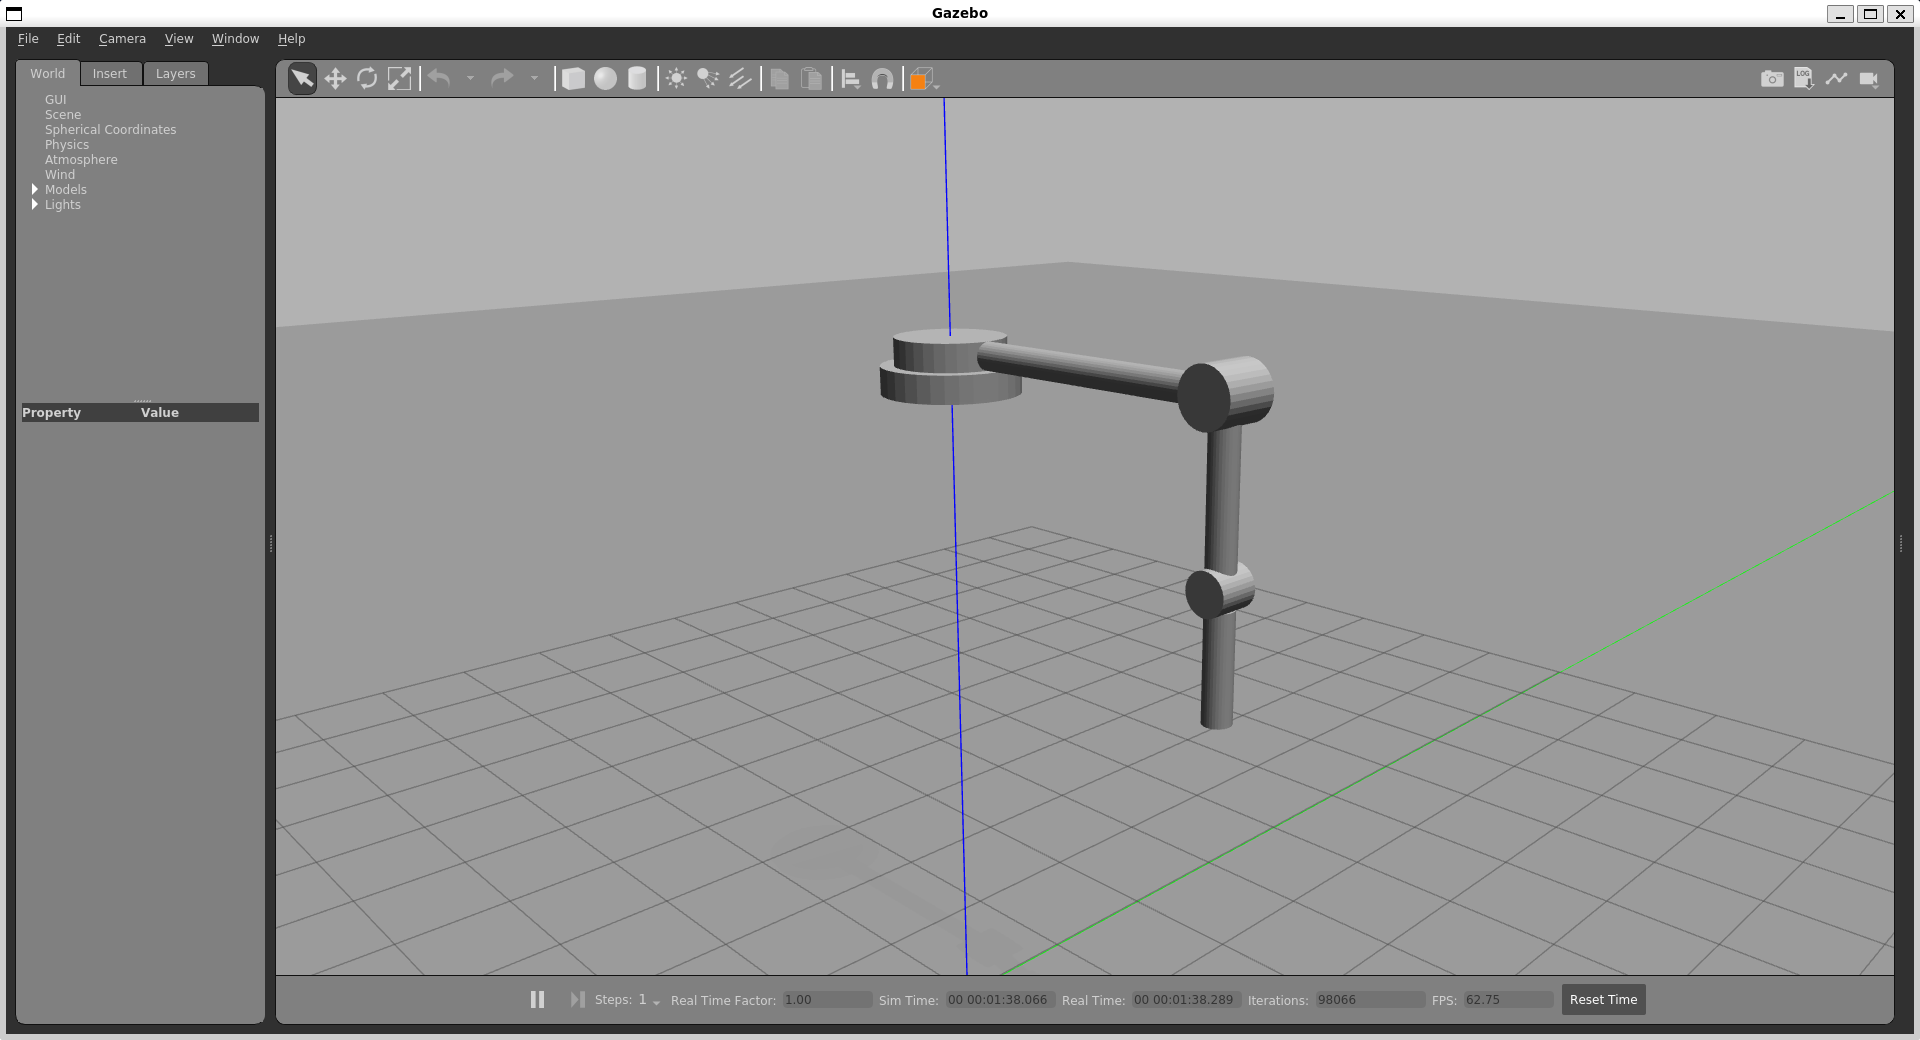
\includegraphics[width=\linewidth]{figures/robotic-arm-gazebo}
        \caption{Gazebo Interface}
    \end{subfigure}
    \hfill
    \begin{subfigure}{0.45\linewidth}
        \centering
        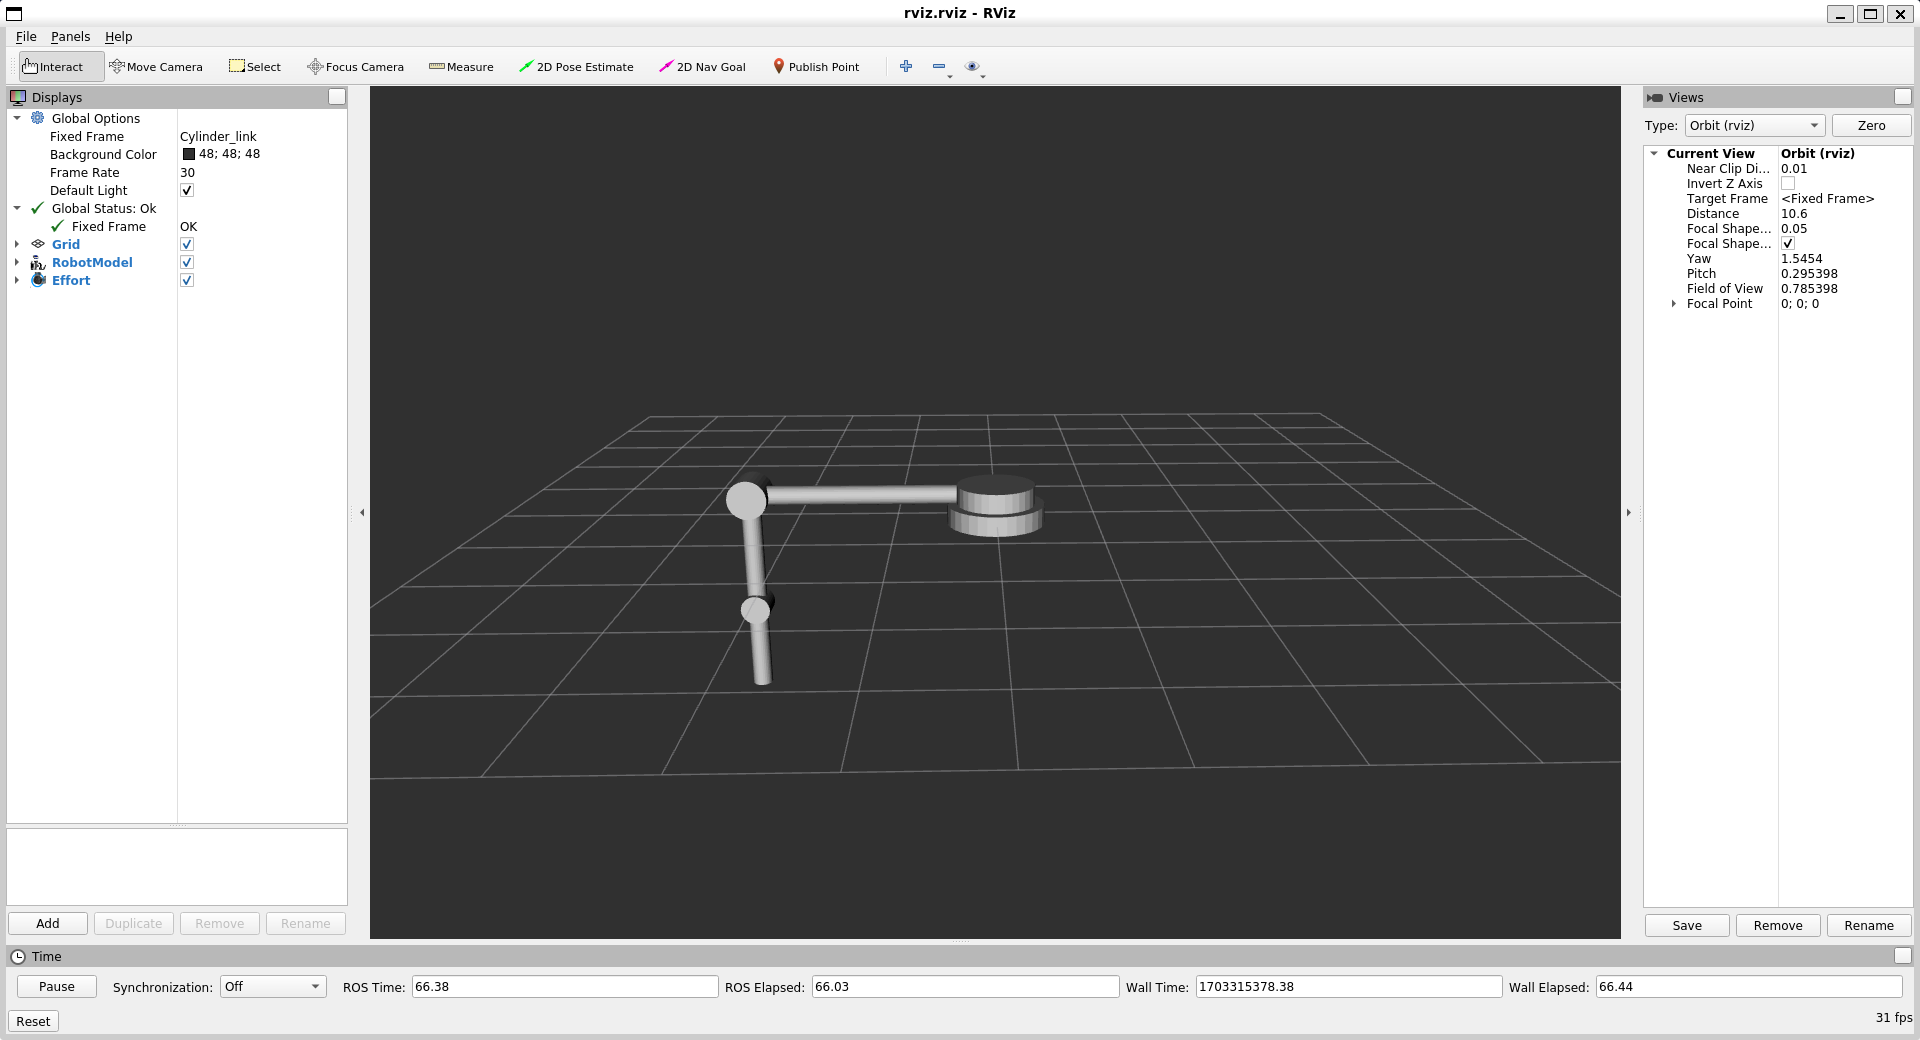
\includegraphics[width=\linewidth]{figures/robotic-arm-rviz}
        \caption{ROS RViz Interface}
    \end{subfigure}
    \hfill
    \caption{Model used for simulation}
    \label{fig:model}
\end{figure}

%利用 Blender 这一商业级三维模型编辑软件,可以非常容易地得到高精度的机械臂三维模型。
%通过将模型三角面化,然后指定材质,即可使用 Phobos 插件比较容易地计算出每个部件的质量和转动惯量。
% 为了简单起见,我们使用具有质量对称轴且与坐标轴对齐的几何形状进行设计,从而得到的惯量张量总是对角矩阵,具体数值如下所示。
Using Blender, a commercial-grade 3D model editing software, we can easily obtain a high-precision 3D model of the robotic arm.
By triangulating the model and assigning materials, the mass and moment of inertia of each part can be calculated relatively easily using the Phobos plug-in.
For the sake of simplicity, we design using a geometry with a mass symmetry axis aligned with the coordinate axis, so that the resulting inertia tensor is always a diagonal matrix, as shown below.
\[
    \begin{aligned}
        I_1 = &
        \begin{bmatrix}
            0.02723 & 0 & 0 \\
            0 & 0.58138 & 0 \\
            0 & 0 & 0.60282 \\
        \end{bmatrix} \\
        I_2 = &
        \begin{bmatrix}
            0.01588 & 0 & 0 \\
            0 & 0.12671 & 0 \\
            0 & 0 & 0.12900 \\
        \end{bmatrix} \\
        I_3 = &
        \begin{bmatrix}
            0.08836 & 0 & 0 \\
            0 & 0.08734 & 0 \\
            0 & 0 & 0.00864 \\
        \end{bmatrix}
    \end{aligned}
\]
 %除此之外,还需要设计用于碰撞检测的几何模型。
% 直接使用网格会造成较大的性能负担,因此通常使用简单的几何形状如长方体等进行计算。
% 导出 URDF 文件后,还需要手动输入一些物理属性,如关节处的电机减速比和关节的阻尼与摩擦系数等。
% 除此之外,还需要在 URDF 中指定 Gazebo 插件等仿真使用的数据。
In addition, a geometric model for collision detection also needs to be designed.
Using the meshes directly will cause a large performance burden, so simple geometric shapes such as cuboids are usually used for calculations.
After exporting the URDF file, it is still needed to manually input some physical properties, such as the motor reduction ratio at the joint and the damping and friction coefficient of the joint.
In addition, data used by simulations such as Gazebo plug-ins also need to be specified in the URDF.

%此后,通过将 URDF 与三维模型文件组织成 ROS 软件包的形式,撰写``.launch''文件,指定控制器和控制器的参数等步骤,即可完成仿真环境的搭建。
% 以下为仿真中使用的``.launch''文件。
Thereafter, by organizing the URDF and 3D model files into a ROS software package, writing a ``.launch'' file, specifying the controller and controller parameters, etc., the simulation environment can be built.
The following is the ``.launch'' file used in the simulation.
\lstinputlisting[language=XML]{../catkin_ws/src/robot_description/launch/gazebo.launch}

\subsection{Simulation Result}

% 我们使用简单的PID控制器对机械臂的前三个转动关节的角度$\theta_{1,2,3}$进行控制。
% 该控制器由 ROS 中的软件包 \emph{ros\_control} 实现。
% 通过将控制器参数载入 ROS 参数服务器,在 Gazebo 中加载控制器插件 \emph{gazebo\_ros\_control},在URDF文件中指定传动信息等操作,即可实现机械臂的控制仿真。

We use a simple PID controller to control the angles $\theta_{1,2,3}$ of the first three rotating joints of the robotic arm.
This controller is implemented by the package \emph{ros\_control} in ROS.
By loading the controller parameters into the ROS parameter server, loading the controller plug-in \emph{gazebo\_ros\_control} in Gazebo, and specifying the transmission information in the URDF file, the control simulation of the robotic arm can be realized.

% 我们为每一个关节分配了根据位置控制扭矩的PID控制器,并根据仿真的结果调整参数。
% 以关节二为例,仿真结果如图\ref{fig:simulated-result}所示。
We assign a PID controller that controls torque based on position to each joint, and adjust the parameters based on the simulation results.
The simulation results are shown in \autoref{fig:simulated-result}.

\begin{figure}[ht]
    \centering
    \begin{subfigure}{0.8\linewidth}
        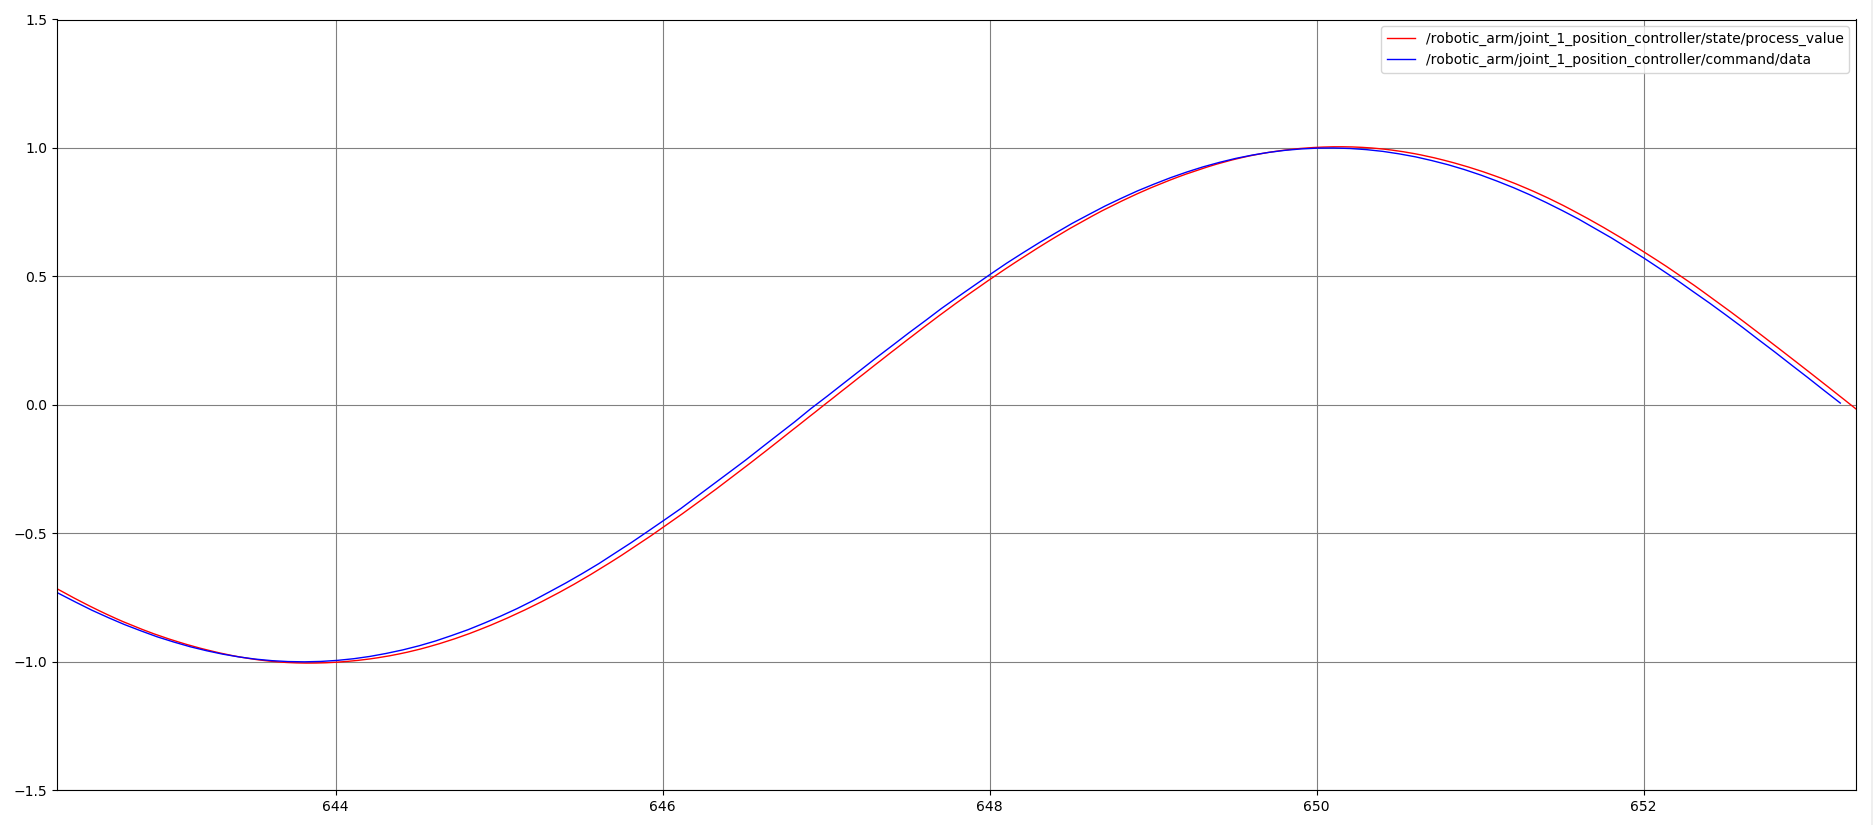
\includegraphics[width=\linewidth]{figures/result-joint-1.PNG}
        \caption{Joint One}
    \end{subfigure}
    \\
    \begin{subfigure}{0.8\linewidth}
        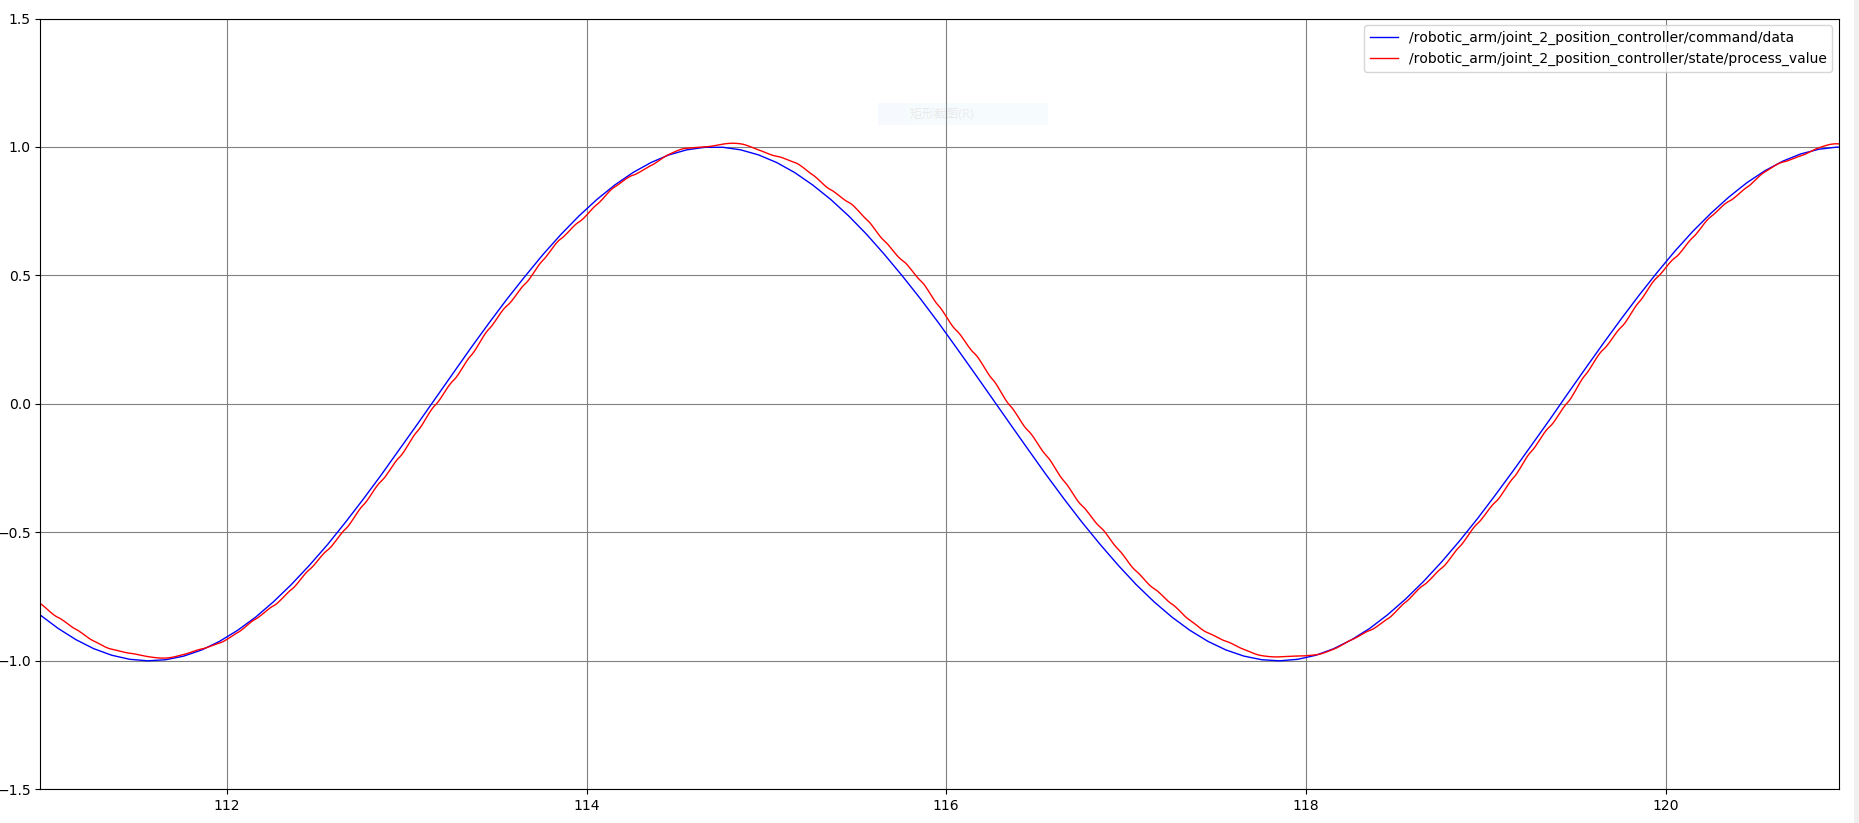
\includegraphics[width=\linewidth]{figures/result-joint-2.PNG}
        \caption{Joint Two}
    \end{subfigure}
    \\
    \begin{subfigure}{0.8\linewidth}
        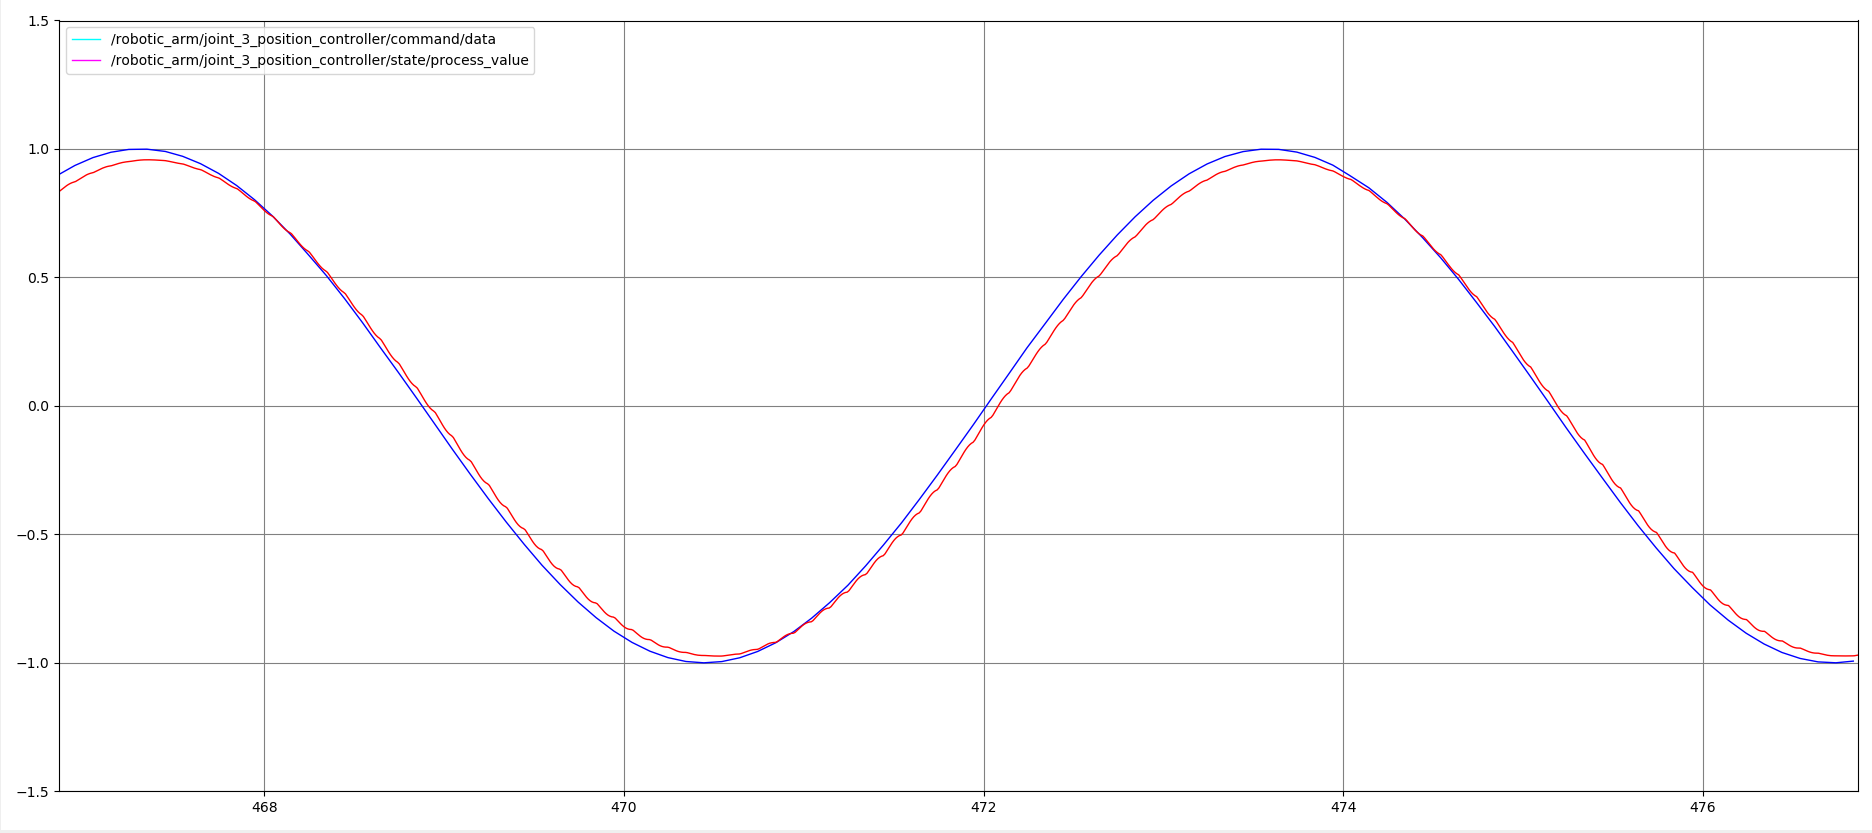
\includegraphics[width=\linewidth]{figures/result-joint-3.PNG}
        \caption{Joint Three}
    \end{subfigure}
    \caption[Simulated results]{Simulated results (Blue lines shows commands and red lines shows actual joint angles)}
    \label{fig:simulated-result}
\end{figure}

The parameters of PID controllers used in simulations are as follows:
\[
    \begin{aligned}
        K_p = & \begin{bmatrix}
            1000 & 0 & 0 \\
            0 & 600 & 0 \\
            0 & 0 & 100 \\
        \end{bmatrix} \\
        K_i = & 0.01 \mathbf I \\
        K_d = & 10 \mathbf I
    \end{aligned}
\]

\end{document}
